% Created by tikzDevice version 0.10.1 on 2018-01-23 16:20:31
% !TEX encoding = UTF-8 Unicode
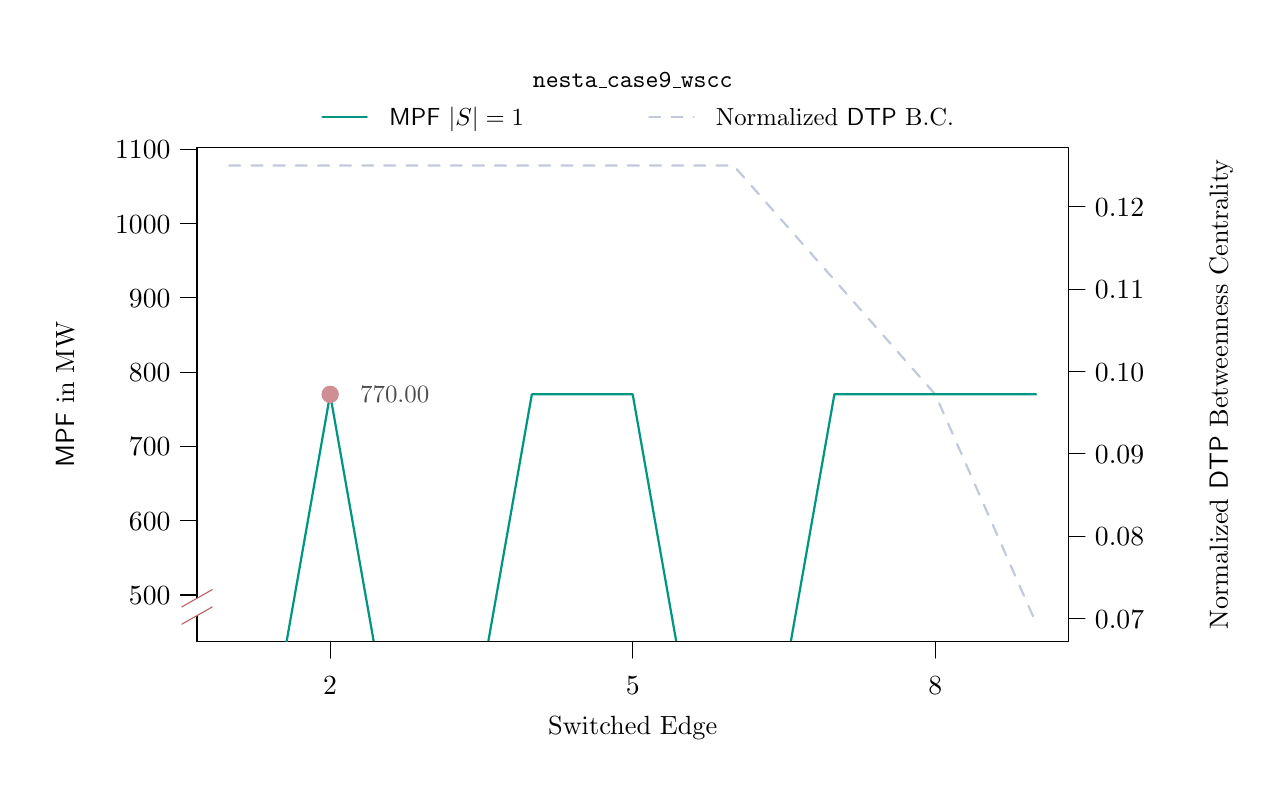
\begin{tikzpicture}[x=1pt,y=1pt]
\definecolor{fillColor}{RGB}{255,255,255}
\path[use as bounding box,fill=fillColor,fill opacity=0.00] (0,0) rectangle (440.85,271.01);
\begin{scope}
\path[clip] (  0.00,  0.00) rectangle (440.85,271.01);
\definecolor{drawColor}{RGB}{193,202,220}

\path[draw=drawColor,line width= 0.8pt,dash pattern=on 4pt off 4pt ,line join=round,line cap=round] ( 72.86,221.20) --
	(109.30,221.20) --
	(145.74,221.20) --
	(182.18,221.20) --
	(218.62,221.20) --
	(255.06,221.20) --
	(291.50,179.85) --
	(327.95,138.51) --
	(364.39, 55.82);
\end{scope}
\begin{scope}
\path[clip] (  0.00,  0.00) rectangle (440.85,271.01);
\definecolor{drawColor}{RGB}{0,0,0}

\path[draw=drawColor,line width= 0.4pt,line join=round,line cap=round] ( 61.20, 49.20) --
	(376.05, 49.20) --
	(376.05,227.81) --
	( 61.20,227.81) --
	( 61.20, 49.20);
\end{scope}
\begin{scope}
\path[clip] (  0.00,  0.00) rectangle (440.85,271.01);
\definecolor{drawColor}{RGB}{0,0,0}

\path[draw=drawColor,line width= 0.4pt,line join=round,line cap=round] (376.05, 57.47) -- (376.05,206.31);

\path[draw=drawColor,line width= 0.4pt,line join=round,line cap=round] (376.05, 57.47) -- (382.05, 57.47);

\path[draw=drawColor,line width= 0.4pt,line join=round,line cap=round] (376.05, 87.24) -- (382.05, 87.24);

\path[draw=drawColor,line width= 0.4pt,line join=round,line cap=round] (376.05,117.01) -- (382.05,117.01);

\path[draw=drawColor,line width= 0.4pt,line join=round,line cap=round] (376.05,146.78) -- (382.05,146.78);

\path[draw=drawColor,line width= 0.4pt,line join=round,line cap=round] (376.05,176.54) -- (382.05,176.54);

\path[draw=drawColor,line width= 0.4pt,line join=round,line cap=round] (376.05,206.31) -- (382.05,206.31);

\node[text=drawColor,anchor=base west,inner sep=0pt, outer sep=0pt, scale=  1.00] at (385.65, 54.03) {0.07};

\node[text=drawColor,anchor=base west,inner sep=0pt, outer sep=0pt, scale=  1.00] at (385.65, 83.79) {0.08};

\node[text=drawColor,anchor=base west,inner sep=0pt, outer sep=0pt, scale=  1.00] at (385.65,113.56) {0.09};

\node[text=drawColor,anchor=base west,inner sep=0pt, outer sep=0pt, scale=  1.00] at (385.65,143.33) {0.10};

\node[text=drawColor,anchor=base west,inner sep=0pt, outer sep=0pt, scale=  1.00] at (385.65,173.10) {0.11};

\node[text=drawColor,anchor=base west,inner sep=0pt, outer sep=0pt, scale=  1.00] at (385.65,202.87) {0.12};
\end{scope}
\begin{scope}
\path[clip] (  0.00,  0.00) rectangle (440.85,271.01);
\definecolor{drawColor}{RGB}{0,150,130}

\path[draw=drawColor,line width= 0.8pt,line join=round,line cap=round] (106.55,238.60) -- (122.57,238.60);
\definecolor{drawColor}{RGB}{193,202,220}

\path[draw=drawColor,line width= 0.8pt,dash pattern=on 4pt off 4pt ,line join=round,line cap=round] (224.63,238.60) -- (240.65,238.60);
\definecolor{drawColor}{RGB}{0,0,0}

\node[text=drawColor,anchor=base,inner sep=0pt, outer sep=0pt, scale=  0.89] at (218.62,249.28) {\texttt{nesta\_case9\_wscc}};

\node[text=drawColor,anchor=base west,inner sep=0pt, outer sep=0pt, scale=  0.89] at (130.58,235.54) {$\mathsf{MPF}~|S|=1$};

\node[text=drawColor,anchor=base west,inner sep=0pt, outer sep=0pt, scale=  0.89] at (248.66,235.54) {Normalized~$\mathsf{DTP}$~B.C.};
\end{scope}
\begin{scope}
\path[clip] (  0.00,  0.00) rectangle (440.85,271.01);
\definecolor{drawColor}{RGB}{0,0,0}

\path[draw=drawColor,line width= 0.4pt,line join=round,line cap=round] ( 61.20, 66.02) -- ( 61.20,227.10);

\path[draw=drawColor,line width= 0.4pt,line join=round,line cap=round] ( 61.20, 66.02) -- ( 55.20, 66.02);

\path[draw=drawColor,line width= 0.4pt,line join=round,line cap=round] ( 61.20, 92.87) -- ( 55.20, 92.87);

\path[draw=drawColor,line width= 0.4pt,line join=round,line cap=round] ( 61.20,119.71) -- ( 55.20,119.71);

\path[draw=drawColor,line width= 0.4pt,line join=round,line cap=round] ( 61.20,146.56) -- ( 55.20,146.56);

\path[draw=drawColor,line width= 0.4pt,line join=round,line cap=round] ( 61.20,173.41) -- ( 55.20,173.41);

\path[draw=drawColor,line width= 0.4pt,line join=round,line cap=round] ( 61.20,200.26) -- ( 55.20,200.26);

\path[draw=drawColor,line width= 0.4pt,line join=round,line cap=round] ( 61.20,227.10) -- ( 55.20,227.10);

\node[text=drawColor,anchor=base east,inner sep=0pt, outer sep=0pt, scale=  1.00] at ( 51.60, 62.57) {500};

\node[text=drawColor,anchor=base east,inner sep=0pt, outer sep=0pt, scale=  1.00] at ( 51.60, 89.42) {600};

\node[text=drawColor,anchor=base east,inner sep=0pt, outer sep=0pt, scale=  1.00] at ( 51.60,116.27) {700};

\node[text=drawColor,anchor=base east,inner sep=0pt, outer sep=0pt, scale=  1.00] at ( 51.60,143.12) {800};

\node[text=drawColor,anchor=base east,inner sep=0pt, outer sep=0pt, scale=  1.00] at ( 51.60,169.96) {900};

\node[text=drawColor,anchor=base east,inner sep=0pt, outer sep=0pt, scale=  1.00] at ( 51.60,196.81) {1000};

\node[text=drawColor,anchor=base east,inner sep=0pt, outer sep=0pt, scale=  1.00] at ( 51.60,223.66) {1100};
\end{scope}
\begin{scope}
\path[clip] (  0.00,  0.00) rectangle (440.85,271.01);
\definecolor{drawColor}{RGB}{255,255,255}
\definecolor{fillColor}{RGB}{255,255,255}

\path[draw=drawColor,line width= 0.4pt,line join=round,line cap=round,fill=fillColor] ( 55.69, 58.58) rectangle ( 66.71, 64.83);
\definecolor{drawColor}{RGB}{188,97,104}

\path[draw=drawColor,line width= 0.4pt,line join=round,line cap=round] ( 55.69, 55.45) -- ( 66.71, 61.70);

\path[draw=drawColor,line width= 0.4pt,line join=round,line cap=round] ( 55.69, 61.70) -- ( 66.71, 67.95);
\end{scope}
\begin{scope}
\path[clip] ( 61.20, 49.20) rectangle (376.05,227.81);
\definecolor{drawColor}{RGB}{0,150,130}

\path[draw=drawColor,line width= 0.8pt,line join=round,line cap=round] ( 84.89,  0.00) --
	(109.30,138.51) --
	(133.72,  0.00);

\path[draw=drawColor,line width= 0.8pt,line join=round,line cap=round] (157.77,  0.00) --
	(182.18,138.51) --
	(218.62,138.51) --
	(243.04,  0.00);

\path[draw=drawColor,line width= 0.8pt,line join=round,line cap=round] (267.09,  0.00) --
	(291.50,138.51) --
	(327.95,138.51) --
	(364.39,138.51);
\end{scope}
\begin{scope}
\path[clip] ( 61.20, 49.20) rectangle (376.05,227.81);
\definecolor{fillColor}{RGB}{207,142,147}

\path[fill=fillColor] (109.30,138.51) circle (  3.15);
\end{scope}
\begin{scope}
\path[clip] ( 61.20, 49.20) rectangle (376.05,227.81);
\definecolor{drawColor}{gray}{0.30}

\node[text=drawColor,anchor=base,inner sep=0pt, outer sep=0pt, scale=  0.90] at (132.62,135.62) {770.00};
\end{scope}
\begin{scope}
\path[clip] (  0.00,  0.00) rectangle (440.85,271.01);
\definecolor{drawColor}{RGB}{0,0,0}

\path[draw=drawColor,line width= 0.4pt,line join=round,line cap=round] (109.30, 49.20) -- (327.95, 49.20);

\path[draw=drawColor,line width= 0.4pt,line join=round,line cap=round] (109.30, 49.20) -- (109.30, 43.20);

\path[draw=drawColor,line width= 0.4pt,line join=round,line cap=round] (218.62, 49.20) -- (218.62, 43.20);

\path[draw=drawColor,line width= 0.4pt,line join=round,line cap=round] (327.95, 49.20) -- (327.95, 43.20);

\node[text=drawColor,anchor=base,inner sep=0pt, outer sep=0pt, scale=  1.00] at (109.30, 30.00) {2};

\node[text=drawColor,anchor=base,inner sep=0pt, outer sep=0pt, scale=  1.00] at (218.62, 30.00) {5};

\node[text=drawColor,anchor=base,inner sep=0pt, outer sep=0pt, scale=  1.00] at (327.95, 30.00) {8};

\node[text=drawColor,anchor=base,inner sep=0pt, outer sep=0pt, scale=  0.95] at (218.62, 15.60) {Switched Edge};

\node[text=drawColor,rotate= 90.00,anchor=base,inner sep=0pt, outer sep=0pt, scale=  0.95] at ( 16.80,138.51) {$\mathsf{MPF}$ in~$\mathrm{MW}$};

\node[text=drawColor,rotate= 90.00,anchor=base,inner sep=0pt, outer sep=0pt, scale=  0.95] at (433.65,138.51) {Normalized~$\mathsf{DTP}$ Betweenness Centrality};
\end{scope}
\end{tikzpicture}
